
\documentclass[a4paper]{article}
\usepackage{epsfig,epic,eepic,amssymb}
\graphicspath{{FIG/}{PS/}}
\usepackage[francais]{babel}
\usepackage[latin1]{inputenc}
\usepackage{amssymb}
\usepackage{moreverb}
\usepackage{listings}
\lstset{language=caml, extendedchars=true}
\newtheorem{theorem}{Theorem}

\usepackage{graphicx}
\usepackage{amsfonts}
\def\C{\mathbb{C}}
\def\N{\mathbb{N}}
\def\Z{\mathbb{Z}}
\def\R{\mathbb{R}}

\begin{document}
\title{TD : l'escalier}
\author{Dominique Michelucci, Universit\'e de Dijon}
\maketitle

Un ensemble $P$ de $n$ points 2D $P_i=(x_i, y_i)$ est donn\'e.
On suppose que tous les points sont dans le quadrant positif~: $x_i \le 0, y_i\le 0$ pour tout $i$. 

On dit que $p_i \le q_i$ ssi $x_i \le x_j$ et $y_i\le y_j$.

Pourquoi cet ordre n'est il que partiel~? 

On appelle escalier de $P$ le sous ensemble des points de $P$ qui sont des minima pour cet ordre.
Il est not\'e $E$, ou $E(P)$.

Donner un exemple o\`u $E$ contient un seul point de $P$.

Donner un exemple o\`u $E=P$.

Proposer des m\'ethodes pour calculer $E(P)$. Les  m\'ethodes de tri sont une source d'inspiration possible~:
il y a des m\'ethodes en $O(n^2)$ et en $O(n\log n)$.

Il y a 2 variantes~: soit on veut juste $E$, soit en plus on veut $E$ "dans l'ordre" ($x$ croissant, par exemple).

R\'eduire le probl\`eme du tri de $X$, $x_i \ge 0$, au probl\`eme de l'escalier.
En d\'eduire que (si les $x_i$ ne sont pas entiers)
l'escalier ne peut \^etre r\'esolu plus vite que $O(n\log n)$.

Remarque: Dickson's lemma: si les $P_i$ sont \`a coordonn\'ees enti\`eres, alors $E(P)$ est fini m\^eme si $E$ est infini. Prouvez le
(En pratique, $E$ bien qu'infini a une description finie.)
Ce lemme est fondamental pour le calcul formel et les bases de Grobner (ce sera vu en M1 info).

\begin{center}
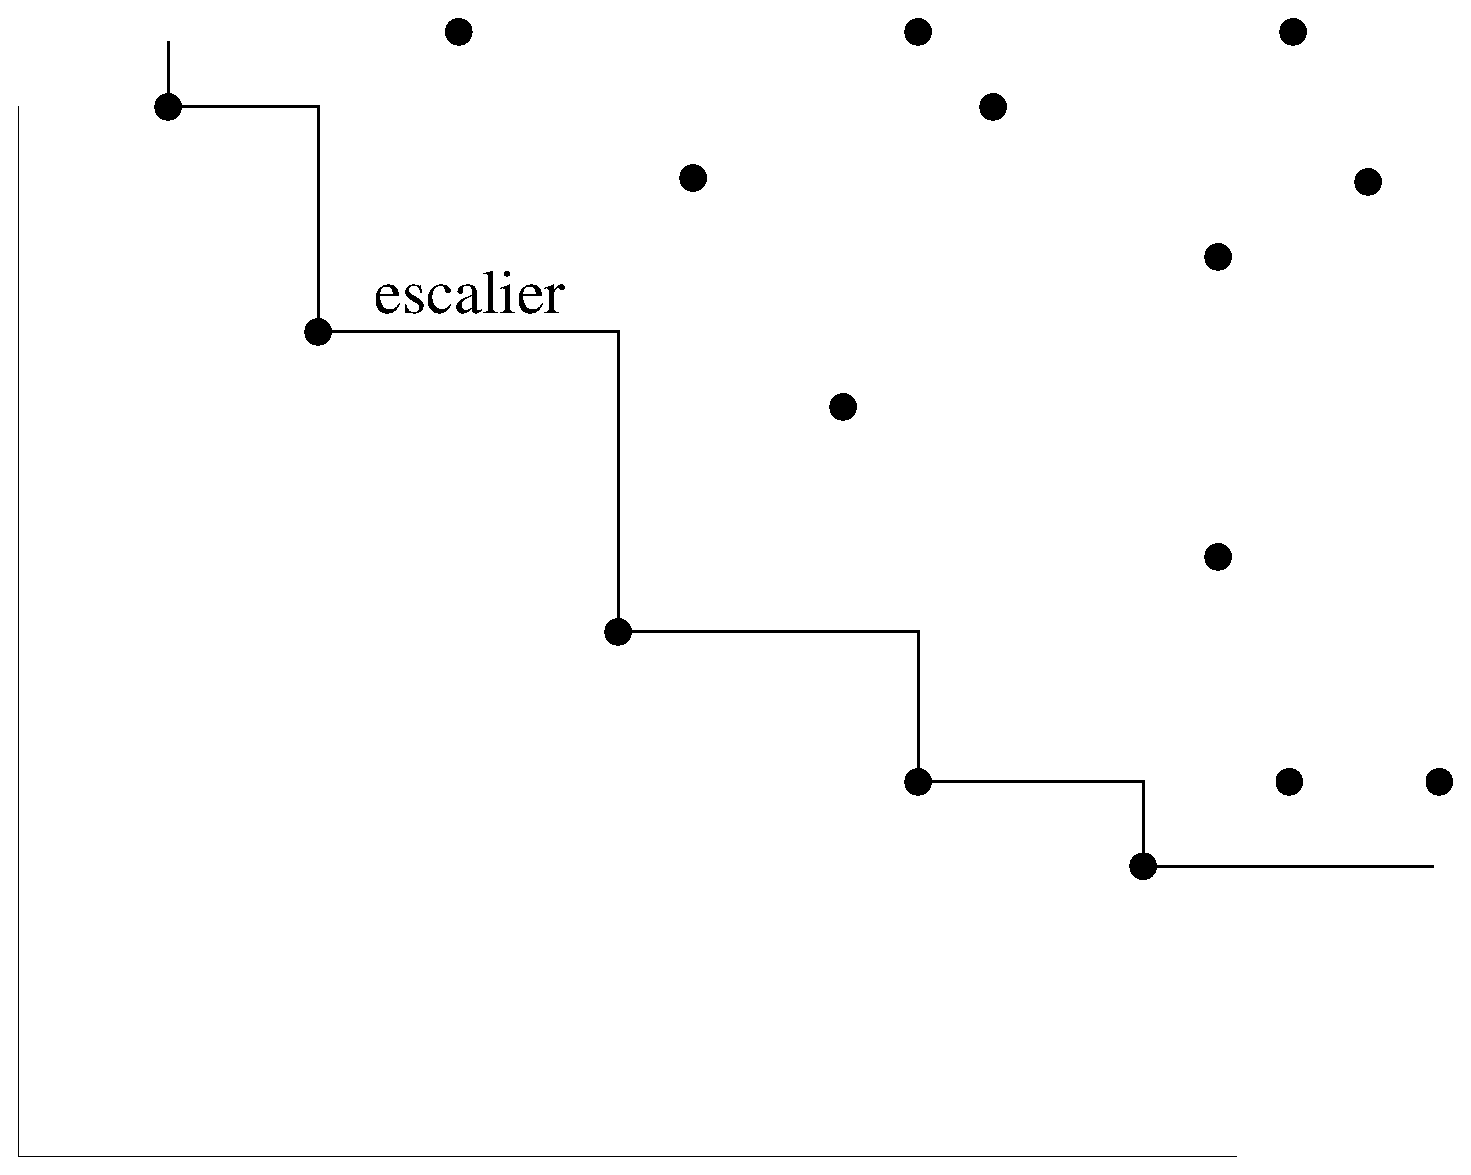
\includegraphics[width=0.6\linewidth]{escalier.eps}
\end{center}

\newpage

Algo quadratique~: comparer tous les $P_i, P_j$. Cet algo ne donne pas la structure.

Algo $O(n\log n)$: trier $P$ par $x$ croissant (pour le m\^eme $x$, par $y$ d\'ecroissant). Balayer $P=(P_1, P_2\ldots P_n)$ ainsi tri\'e, par indice croissant,
en g\'erant $Y$, un $y$ minimal qui ne peut que d\'ecro\^itre
au cours de l'algo~: si le point $P_k$ est au dessus de $Y$, l'\'eliminer. S'il est dessous, l'ins\'erer en fin de l'escalier, et mettre $Y$ \`a jour~: $Y\leftarrow P_k.y$.

Algo $O(n\log n)$: s'inspirer du quicksort: le modifier pour \'eliminer les points plus grands que le piv\^ot.
Attention \`a l'utilisation de 2 ordres distincts: l'ordre partiel, et l'ordre sur les $x$...

Algo $O(n\log n)$: S'inspirer de tri par fusion: il faut fusionner 2 escaliers (ordonn\'es par $x$ croissant).

R\'eduire le probl\`eme du tri de $X$, $x_i \ge 0$, au probl\`eme de l'escalier. 
En d\'eduire que (si les $x_i$ ne sont pas entiers)
l'escalier ne peut \^etre r\'esolu plus vite que $O(n\log n)$.

R: Consid\'erer $P_i=(x_i, y_i = S- x_i)$ o\`u $S=  \max x_i$. Alors $E=P$.
M\^eme genre de preuve que celle qui montre que le calcul de l'enveloppe convexe ne peut \^etre faite plus vite que en $O(n\log n)$.

Remarque: Dickson's lemma: si les $P_i$ sont \`a coordonn\'ees enti\`eres, alors $E(P)$ est fini m\^eme si $E$ est infini. Prouvez le
(En pratique, $E$ bien qu'infini a une description finie.)

Consid\'erer le point (ou un des points) $P_q$ tel que $x_q+y_q$ est maximum. Ce point est dans $E$, et 
"\'elimine" une partie des points de $P$, les points $P_k$ tels que $x_q \le x_k$ et $y_q \le y_k$. 
Il reste des points de $P$ dans 2 bandes, une horizontale entre $y=0 $ et $y=y_q$, et une bande verticale
entre $x=0$ et $x=x_q$.
La bande horizontale a une quantit\'e finie de droites  horizontales enti\`eres: donc l'escalier qui la concerne
ne peut pas contenir davantage de points. Idem pour la bande verticale.
Se g\'en\'eralise en dimension quelconque (finie, quand m\^eme).
\end{document}
